\section{機器人模型}
\label{sec:robot}

\subsection{外觀與尺寸}


為了方便描述機器人的外觀尺寸，因此定義一個外觀的「像素」單位：$1 \text{px} = \frac{1}{16} \text{公尺}$。
機器人總高 28 px（即 1.75 公尺）、總寬 14 px（0.875 公尺）、厚 5 px（0.3125 公尺）。

機器人可以分成頭、脖子、軀幹、左右上臂、左右前臂、左右大腿、左右小腿共 11 個部位（圖~\ref{fig:robot-look}）。
每個部位都有一個局部坐標系（LCS），原點為關節位置，$+y$ 軸為向上、$+z$ 軸為面向前方、$+x$ 軸為向左。

\begin{figure}[htbp]
    \centering
    \begin{subfigure}[t]{.32\textwidth}
        \centering
        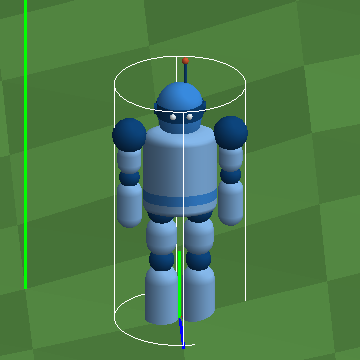
\includegraphics[width=\linewidth]{docs/figures/robot-front.png}
        \caption{正面}
    \end{subfigure}\hfill
    \begin{subfigure}[t]{.32\textwidth}
        \centering
        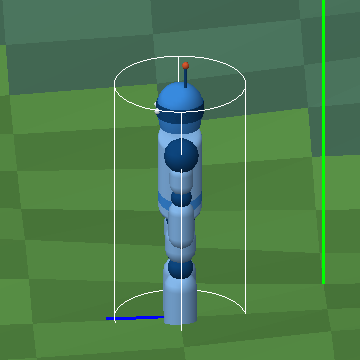
\includegraphics[width=\linewidth]{docs/figures/robot-side.png}
        \caption{側面}
    \end{subfigure}\hfill
    \begin{subfigure}[t]{.32\textwidth}
        \centering
        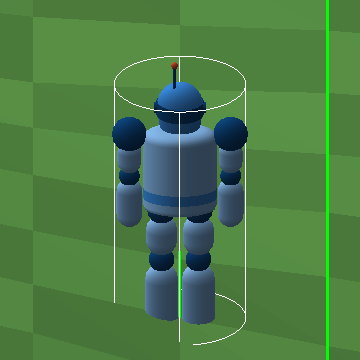
\includegraphics[width=\linewidth]{docs/figures/robot-back.png}
        \caption{背面}
    \end{subfigure}
    \caption{機器人的外觀}
    \label{fig:robot-look}
\end{figure}

而每個部位的外觀模型都是由一組三角形網格（Mesh）組成的。
首先以直線、圓弧與 Bézier 曲線在 $+x y$ 半平面上描述 2D 剖面，
再由 \lstinline|MeshBuilder| 組合，繞 $y$ 軸旋轉成旋轉體（lathe），
接著使用 $4 \times 4$ 齊次矩陣進行平移、旋轉與縮放等變換，最後得到部位的網格。

只塗上純色時，同一個部位的每個面顏色都一樣，看不出表面的起伏與立體感，因此對每個三角形的顏色乘上一個依法向量計算的亮度倍率。
參考 Inigo Quilez 在 YouTube 上的教學，
表面的亮度可以由單位法向量 $\mathbf{n}$ 與指向太陽的單位向量 $\mathbf{l}$ 的內積得到，越正對太陽的面越亮；
但直接取 $\max(0, \mathbf{n} \cdot \mathbf{l})$ 時，背對太陽的面會全部變成同一個暗色，
所以使用 Half-Lambert 演算法，把內積從 $[-1, 1]$ 映射到 $[0, 1]$ 再平方：
$$
    b(\mathbf{n}) = \left( \tfrac{1}{2}\, \mathbf{n} \cdot \mathbf{l} + \tfrac{1}{2} \right)^2, \qquad
    s(\mathbf{n}) = \min\!\left( 1,\; 0.32 + 0.68 \times 0.9 \times \frac{b(\mathbf{n})}{b(\hat{\mathbf{y}})} \right).
$$
接著定義亮度倍率 $s$ 最暗為 0.32（正背對太陽的面），
平地（$\mathbf{n} = \hat{\mathbf{y}} = \left[0, 1, 0\right]^\top$）的亮度倍率為 0.9，讓面對太陽的斜面比平地更亮。


\subsection{場景圖}
\label{sec:scene-graph}

機器人的場景圖如圖~\ref{fig:scene-graph}。
每個節點是一根骨頭（bone），記錄它的父節點、關節在父節點座標系中的位置（pivot），以及可轉動的角度範圍。
根節點 root 本身沒有關節，只帶有一個隨姿勢改變的平移量 rootOffset，用來決定髖部離地的高度。
軀幹的原點在髖部中央，雙腿從髖部往下、雙臂從肩膀往下延伸，脖子接在軀幹頂端，頭再接在脖子上。

\begin{figure}[htbp]
    \centering
    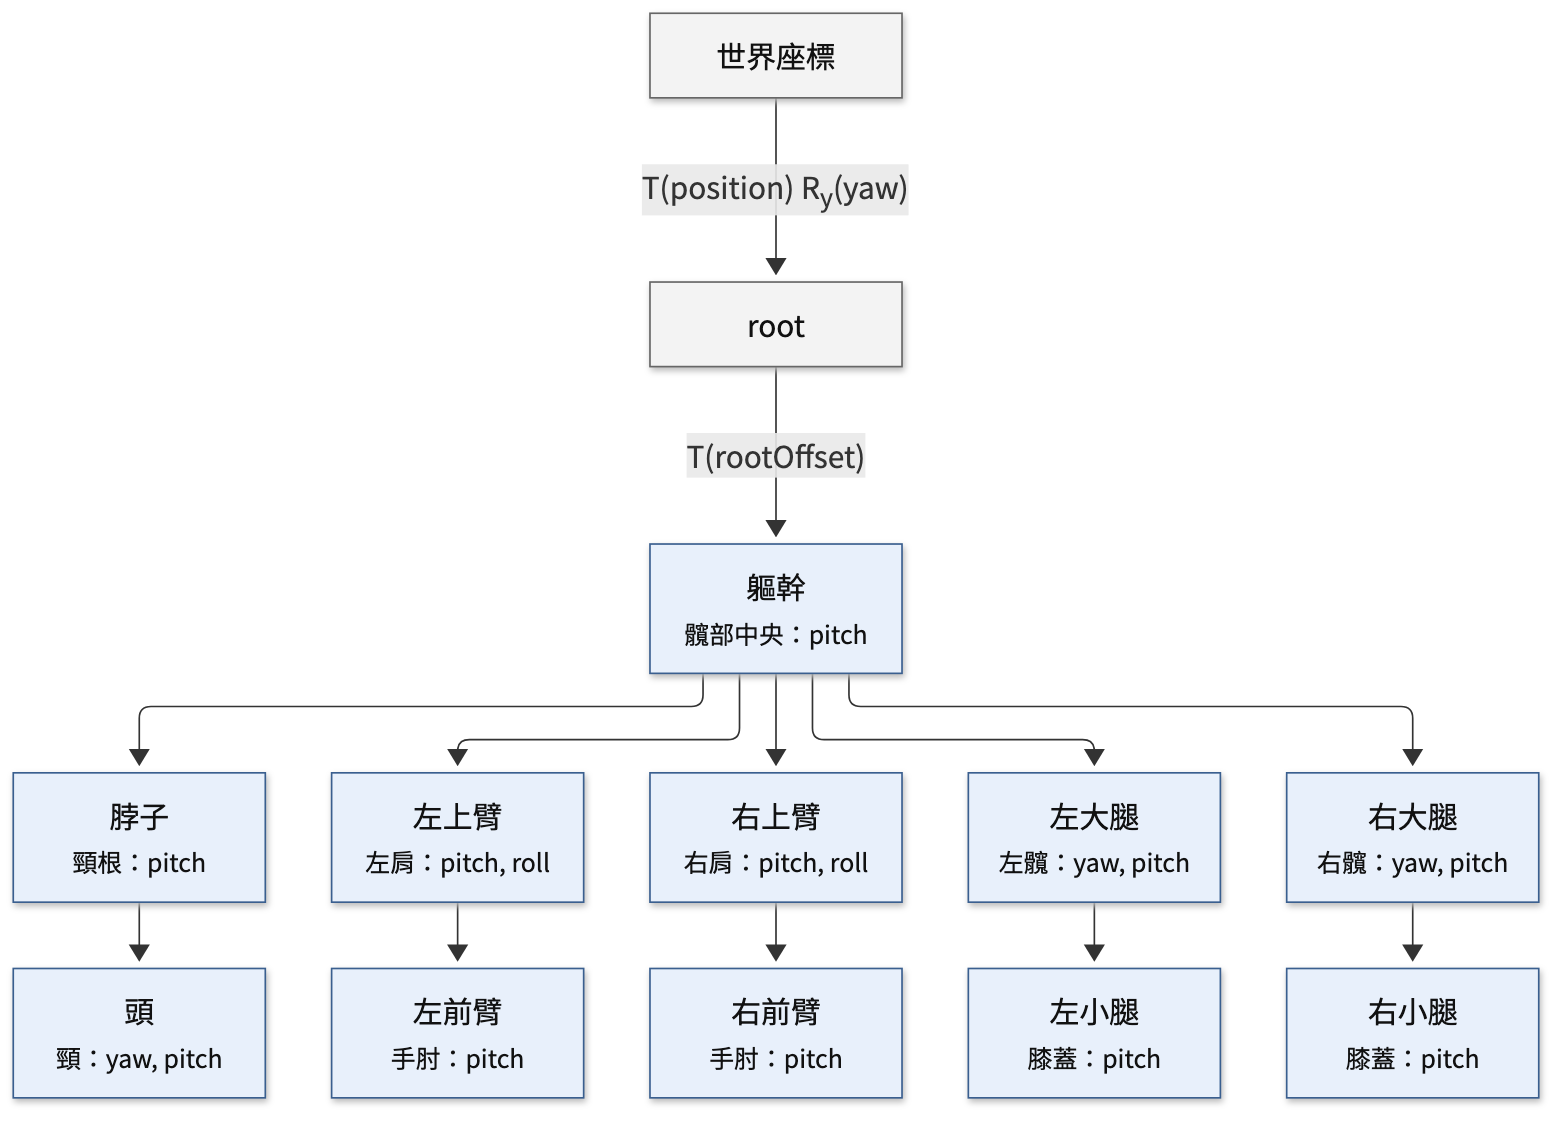
\includegraphics[width=.8\textwidth]{docs/figures/ch03_scene-graph.png}
    \caption{機器人的場景圖，節點下方為連接父節點的關節與其可轉動的軸}
    \label{fig:scene-graph}
\end{figure}

\subsection{關節自由度}
\label{sec:dof}

每個關節最多有 yaw（繞 $y$ 軸）、pitch（繞 $-x$ 軸）、roll（繞 $z$ 軸）三個旋轉自由度；角度範圍上下限相同的軸視為鎖住，不算一個自由度。
骨頭在靜止姿勢時面向 $+z$，pitch 取 $-x$ 為轉軸，正值就是往前抬起，與視線的 pitch 方向一致。
各關節的自由度與角度範圍如表~\ref{tab:dof}，角度範圍以左側為準，右側的 yaw 與 roll 範圍左右對稱、正負相反。
四肢共 12 個自由度，加上軀幹、頭的 4 個，機器人身上共有 15 個旋轉自由度；
另外整隻機器人在世界中還有位置 $(x, y, z)$ 與朝向 yaw 共 4 個自由度。

\begin{table}[H]
    \centering
    \caption{關節的自由度與角度範圍（「—」表示鎖住）}
    \label{tab:dof}
    \small
    \begin{tabular}{lcccc}
        \toprule
        關節       & yaw                       & pitch                      & roll                     & 自由度 \\
        \midrule
        軀幹（髖部中央） & —                         & $-45^\circ \sim 45^\circ$  & —                        & 1   \\
        脖子（頸根）   & —                         & —                          & —                        & 0   \\
        頭（頸）     & $-70^\circ \sim 70^\circ$ & $-60^\circ \sim 50^\circ$  & —                        & 2   \\
        上臂（肩膀）×2 & —                         & $-60^\circ \sim 200^\circ$ & $0^\circ \sim 170^\circ$ & 2   \\
        前臂（手肘）×2 & —                         & $0^\circ \sim 145^\circ$   & —                        & 1   \\
        大腿（髖）×2  & $0^\circ \sim 45^\circ$   & $-30^\circ \sim 120^\circ$ & —                        & 2   \\
        小腿（膝蓋）×2 & —                         & $-140 \sim 0$              & —                        & 1   \\
        \bottomrule
    \end{tabular}
\end{table}

\subsection{階層繪製}

% TODO: 重寫小節

每個關節先平移到關節位置，再旋轉，子節點都畫在旋轉後的座標系裡。
程式依同樣的順序計算每根骨頭的變換矩陣，骨頭 $i$ 的矩陣為
$$
    \begin{cases}
        M_{\text{root}} = M_0 = T(\text{rootOffset}), \\
        M_i = M_{\text{parent}(i)} T(\text{pivot}_i)
        R_y(\text{yaw}_i) R_{-x}(\text{pitch}_i) R_z(\text{roll}_i), i \neq \text{root}.
    \end{cases}
$$
其中 root 的矩陣為 $T(\text{rootOffset})$。骨頭依加入的順序儲存，父節點一定排在子節點前面，所以只要從頭到尾走一遍就能算出所有矩陣，不需要遞迴。
計算前會先把姿勢中的每個角度限制在表~\ref{tab:dof} 的範圍內，因此不論動畫怎麼疊加，關節都不會轉到不合理的角度。

繪製時先以 \lstinline|glTranslatef|、\lstinline|glRotatef| 移到機器人的位置與朝向，
再對每根骨頭 \lstinline|glPushMatrix|、\lstinline|glMultMatrixf(|$M_i$\lstinline|)|、畫出網格、\lstinline|glPopMatrix|。
矩陣與 OpenGL 一樣採用行向量、右乘與 column-major 儲存，可以直接交給 \lstinline|glMultMatrixf|。

同一組矩陣也用在模擬中：頭上的眼睛是一個標記點（marker），以頭的矩陣轉換它的局部座標，就得到眼睛在世界中的位置，相機便以此為焦點。
這部分寫在不依賴 OpenGL 的 \lstinline|world| 模組裡，因此模擬與繪製共用同一份骨架。
